% Documentation of the Perceptron Project
% Subject: Digitaldesign at the Ernst-Abbe-Hochschule Jena
% Author: Fabian Franz

% Packages and Modules
\documentclass{article}
\usepackage{array}
\usepackage{amsmath}
\usepackage{hyperref}
\usepackage{graphicx}
\usepackage{circuitikz}
\usepackage[english]{babel}
\usepackage[utf8]{inputenc}
\usepackage[a4paper, margin=1in]{geometry}
\usepackage{tikz}
\usepackage{float}
\usepackage{mathrsfs}
\usepackage[section]{placeins}
\usepackage{listings}
\usepackage{xcolor}
\usepackage{pdfpages}
\usepackage{etoolbox}

% VHDL
\lstdefinelanguage{VHDL}{
    morekeywords=[1]{
        library,use,all,entity,is,port,in,out,end,architecture,of,if,then,signal,
        begin,and,elsif,others,process,downto,variable,else,range,to,for,loop,wait,
        type,generic,map,generate,layer_resolvers,layer_ad_1D,layer_arr_2D,layer_resolver,perceptron
        },
    morekeywords=[2]{ % name
        behaviour,beh_process,input_process,layer_resolvers_inst,perceptron_arr_inst,
        layer_resolvers_inst,check_beh
        },
    morekeywords=[3]{ % std
        integer,unsigned,std_logic_vector,arr_16_times_16,arr_16_times_7,arr_16_times_4,
        real
    },
    morekeywords=[4]{ % number
        0,1,2,3,4,5,6,7,8,9
    },
    morekeywords=[5]{ % function
        shift_right,rising_edge,to_integer,stop,to_unsigned
    },
  morecomment=[l]--
}
\colorlet{keyword}{red!100!black!80}
\colorlet{comment}{gray!90!black!90}
\colorlet{name}{yellow!90!black!90}
\colorlet{std}{cyan!90!black!80}
\colorlet{number}{purple!90!black!90}
\colorlet{function}{green!70!black!90}
\lstdefinestyle{vhdl}{
  language     = VHDL,
  basicstyle   = \ttfamily,
  keywordstyle = [1]\color{keyword}\bfseries,
  keywordstyle = [2]\color{name}\bfseries,
  keywordstyle = [3]\color{std}\bfseries,
  keywordstyle = [4]\color{number}\bfseries,
  keywordstyle = [5]\color{function}\bfseries,
  commentstyle = \color{comment}
}
\lstdefinestyle{myCustomMatlabStyle}{
  language=VHDL,
  numbers=left,
  stepnumber=1,
  numbersep=8pt,
  tabsize=4,
  showspaces=false,
  showstringspaces=false,
}

% Tikz config
\usetikzlibrary{calc}
\usetikzlibrary{positioning}

% Graphic config
\graphicspath{{./images/}}
\usetikzlibrary{shapes,arrows}
\numberwithin{equation}{section}

% Equation conditions
\newenvironment{conditions}
{\par\vspace{\abovedisplayskip}
\noindent\begin{tabular}{>{$}l<{$} @{${}={}$} l}}
        {\end{tabular}\par\vspace{\belowdisplayskip}}

% Title
\title{Synthese eines Asynchronen Multilayer Perceptron auf einem FPGA}
\author{Fabian Franz, Matr. Nr.: 644414}
\date{Juli 2021}

% Start of the document
\begin{document}
\maketitle

\pagebreak
\tableofcontents
\pagebreak

% Introduction
\section{Einführung}
Dieses Projekt hat den Anspruch, ein effizientes neuronales Netzwerk auf einem FPGA zu
entwerfen. Dazu geben die nächsten Abschnitte eine kurze Einführung in die grundlegenden
Prinzipien, wie ein solches neuronales Netz modelliert werden kann.

\subsection{Perceptron}
Ein Perzeptron beschreibt ein Modell einer biologischen menschlichen Zelle in
Computerdomäne. Dieses Perzeptron kann mit der folgenden Grafik beschrieben und mathematisch
formuliert werden:

\begin{figure}[htbp]
    \begin{center}
        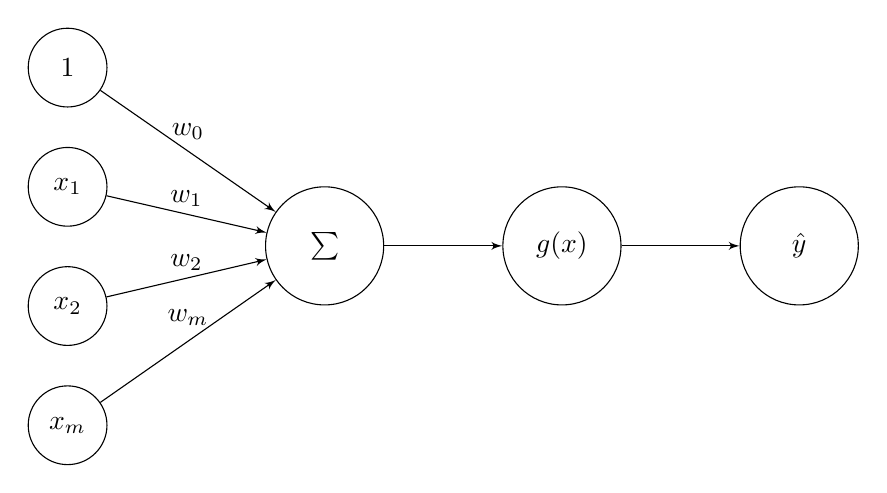
\begin{tikzpicture} [>=latex', node distance = 2cm]
            % Set primary nodes
            \tikzset{
                entity/.style={
                        rectangle,
                        draw
                    }
            }
            \tikzset{
                inputNode/.style={
                        draw,
                        circle,
                        minimum height=1cm
                    }
            }
            \tikzset{
                sumNode/.style={
                        draw,
                        circle,
                        minimum height=1.5cm
                    }
            }
            \tikzset{
                activationNode/.style={
                        draw,
                        circle,
                        minimum height=1.5cm
                    }
            }
            \tikzset{
                outNode/.style={
                        draw,
                        circle,
                        minimum height=1.5cm
                    }
            }
            % Placing nodes
            \node[inputNode](bias){$1$};
            \node[inputNode, below = 0.5cm of bias](x1){$x_1$};
            \node[inputNode, below = 0.5cm of x1](x2){$x_2$};
            \node[inputNode, below = 0.5cm of x2](xm){$x_m$};
            \node[sumNode, right = 2cm of x1, yshift = -0.75cm](sum){$\sum$};
            \node[activationNode, right = 1.5cm of sum](gx){$g(x)$};
            \node[outNode, right = 1.5cm of gx](out){$\hat y$};
            % Placing arrows
            \draw[->](bias) edge node[yshift = 0.25cm]{$w_0$} (sum);
            \draw[->](x1) edge node[yshift = 0.2cm]{$w_1$} (sum);
            \draw[->](x2) edge node[yshift = 0.2cm]{$w_2$} (sum);
            \draw[->](xm) edge node[yshift = 0.3cm]{$w_m$} (sum);
            \draw[->](sum) edge (gx);
            \draw[->](gx) edge (out);
        \end{tikzpicture}
    \end{center}
    \caption{Model des Perzeptron}
\end{figure}
\begin{equation}
    \hat y = g \Bigg( w_0 + \sum_{i=1}^{m}x_i w_i \Bigg)
\end{equation}
Mit:
\begin{conditions}
    g & Aktivierungsfunktion \\
    w_o & Bias
\end{conditions}
In Vektor form:
\begin{equation}
    \hat y = g(W_0 + X^TW)
\end{equation}
Mit:
\begin{conditions}
    W & $\begin{pmatrix} w_1 \\ \vdots \\ w_m \end{pmatrix}$ , X = $\begin{pmatrix} x_1 \\ \vdots \\ x_m \end{pmatrix}$
\end{conditions}
Wie man sieht, wird in einem conventionellen Multilayer-Perzeptron jeder Eingang mit einer
ent-sprechenden Gewichtung multipliziert. Es ist zu erkennen, dass die Umsetzung
eines solchen Perzeptrons von einer gegebenen Hardwarearchitektur wie GPUs oder 
Matrix-Multiplizier-Einheiten abgearbeitet werden kann.

\subsection{Aktivierungsfunktion}
Die Aktivierungsfunktion eines Perzeptrons hat den Zweck, das
Verhalten des Perzeptrons als Reaktion auf äußere Reize zu beeinflussen. Es gibt 
verschiedene Arten von Aktivierungsfunktionen, die für verschiedene Zwecke verwendet 
werden können.

\pagebreak
\section{Design Übersicht}
\subsection{Top Level}
Die Hardware dieses Projekts besteht aus einem 32-Bit-Mikrocontroller namens SAM D21/DA1 und einem
Zyklon 10 FPGA. Beide Chips sind auf einem Board platziert, dem sogenannten Arduino Vidor 4000. Dieses Board
kommt mit einer USB-Schnittstelle, die die Kommunikation zwischen dem Frontend (PC) und
der ausführenden Hardware realisiert. Die Abbildung \ref{fig:abstractHardwareDescription} zeigt das
abstrakte Hardwaremodell. Dieses Modell zeigt das erwähnte Frontend und die Hardware, aber auch den
"Top Level Resolver", der die Daten entweder an den Speicher verteilt, oder die neuen Einstellungen 
für die einzelnen Perceptron-Aktivierungsfunktionen. Im konreten Modell werden insgesamt
16 Schichten mit 16 Perzeptronen pro Schicht realisiert. Der Einfachheit halber sind die 
Takt- und Reset-Signale für jedes einzelne Modul in der Abbildung nicht dargestellt.

% Top Level Hardware Model Diagram
\begin{figure}[htbp]
    \begin{center}
        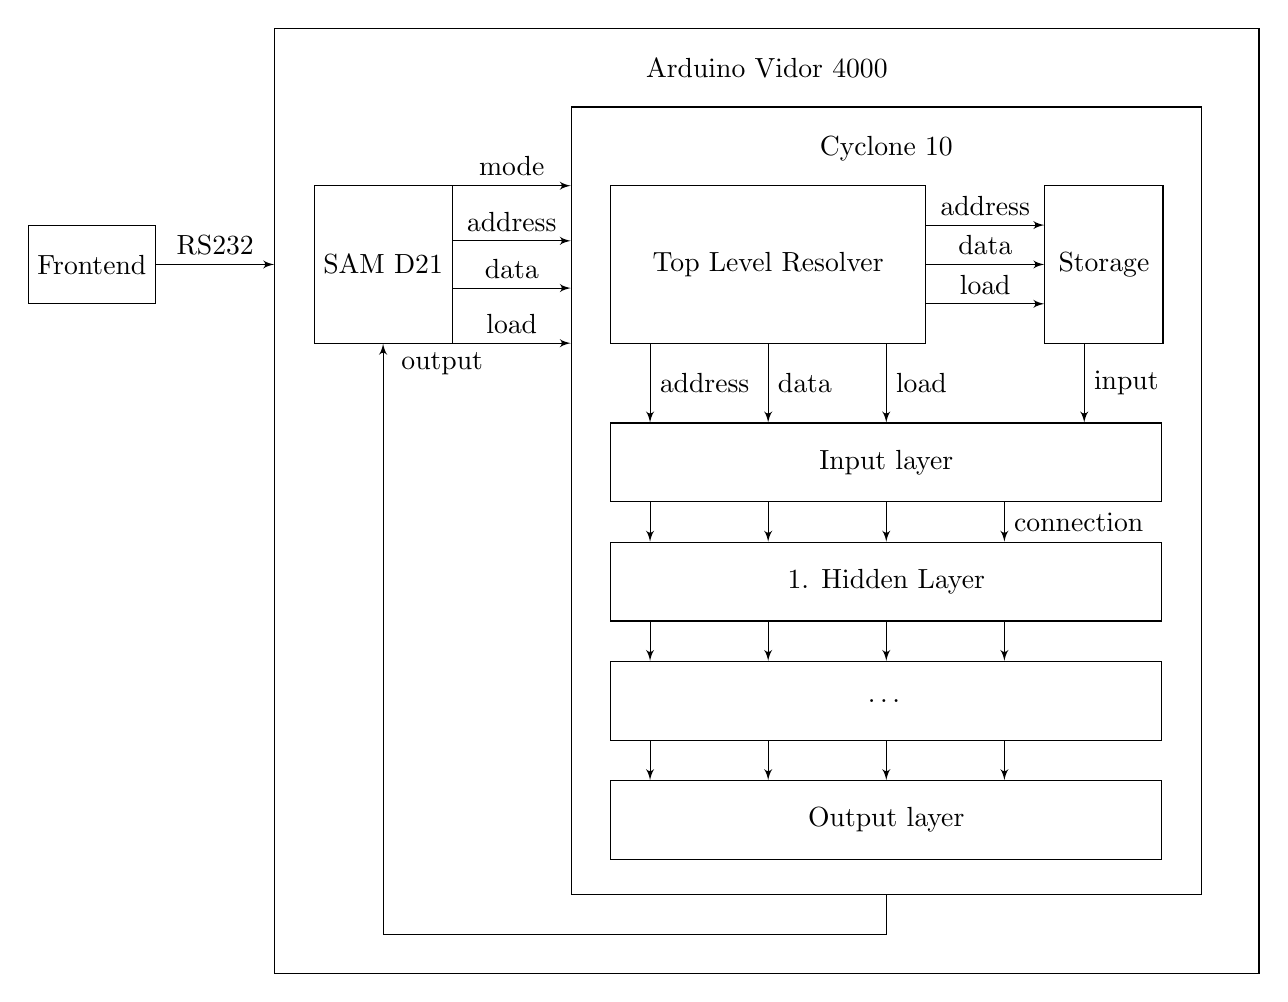
\begin{tikzpicture} [>=latex', node distance = 2cm]
            % Set primary nodes
            \tikzset{
                entity/.style={
                        rectangle,
                        draw
                    }
            }
            \tikzset{
                frontendNode/.style={
                        draw,
                        rectangle,
                        minimum height=1cm,
                        minimum width=1.5cm,
                    }
            }
            \tikzset{
                samd21Node/.style={
                        draw,
                        rectangle,
                        minimum height=2cm,
                        minimum width=1.5cm,
                    }
            }
            \tikzset{
                vidorNode/.style={
                        draw,
                        rectangle,
                        minimum height=12cm,
                        minimum width=12.5cm,
                        text depth = 11cm
                    }
            }
            \tikzset{
                fpgaNode/.style={
                        draw,
                        rectangle,
                        minimum height=10cm,
                        minimum width=8cm,
                        text depth = 9cm
                    }
            }
            \tikzset{
                resolverNode/.style={
                        draw,
                        rectangle,
                        minimum height=2cm,
                        minimum width=4cm
                    }
            }
            \tikzset{
                storageNode/.style={
                        draw,
                        rectangle,
                        minimum height=2cm,
                        minimum width=1.5cm
                    }
            }
            \tikzset{
                layerNode/.style={
                        draw,
                        rectangle,
                        minimum height=1cm,
                        minimum width=7cm
                    }
            }
            \tikzset{
                arrow/.style={
                        thick,
                        ->,
                        >=sealth
                    }
            }
            % Configure arrows
            \tikzstyle{arrow} = [thick, ->, >=stealth]
            % Placing nodes
            \node[frontendNode](frontend){Frontend};
            \node[vidorNode, right = 1.5cm of frontend, yshift = -3cm](vidor){Arduino Vidor 4000};
            \node[samd21Node, right = 2cm of frontend](samd21){SAM D21};
            \node[fpgaNode, right = 1.5cm of samd21, yshift = -3cm](fpga){Cyclone 10};
            \node[resolverNode, right = 2cm of samd21](resolver){Top Level Resolver};
            \node[storageNode, right = 1.5cm of resolver](storage){Storage};
            \node[layerNode, below = 1cm of resolver, xshift = 1.5cm](input){Input layer};
            \node[layerNode, below = 0.5cm of input](hidden1){1. Hidden Layer};
            \node[layerNode, below = 0.5cm of hidden1](hidden2){\dots};
            \node[layerNode, below = 0.5cm of hidden2](output){Output layer};
            % Draw arrows
            \draw[->](frontend.east) -- ++(1.5,0) node[midway,above]{RS232};
            \draw[->](samd21.east) ++(0,1) -- ++(1.5,0) node[midway,above]{mode};
            \draw[->](samd21.east) ++(0,0.3) -- ++(1.5,0) node[midway,above]{address};
            \draw[->](samd21.east) ++(0,-0.3) -- ++(1.5,0) node[midway,above]{data};
            \draw[->](samd21.east) ++(0,-1) -- ++(1.5,0) node[midway,above]{load};
            \draw[->](resolver.east) ++(0,0.5) -- ++(1.5,0) node[midway,above]{address};
            \draw[->](resolver.east) ++(0,0) -- ++(1.5,0) node[midway,above]{data};
            \draw[->](resolver.east) ++(0,-0.5) -- ++(1.5,0) node[midway,above]{load};
            \draw[->](resolver.south) ++(-1.5,0) -- ++(0,-1) node[midway,sloped,right, rotate=90]{address};
            \draw[->](resolver.south) ++(0,0) -- ++(0,-1) node[midway,sloped,right, rotate=90]{data};
            \draw[->](resolver.south) ++(1.5,0) -- ++(0,-1) node[midway,sloped,right, rotate=90]{load};
            \draw[->](storage.south) ++(-0.25,0) -- ++(0,-1) node[midway,sloped,right, rotate=90]{input};
            \draw[->](input.south) ++(-3,0) -- ++(0,-0.5);
            \draw[->](input.south) ++(-1.5,0) -- ++(0,-0.5);
            \draw[->](input.south) ++(0,0) -- ++(0,-0.5);
            \draw[->](input.south) ++(1.5,0) -- ++(0,-0.5) node[midway,sloped,right, rotate=90]{connection};
            \draw[->](hidden1.south) ++(-3,0) -- ++(0,-0.5);
            \draw[->](hidden1.south) ++(-1.5,0) -- ++(0,-0.5);
            \draw[->](hidden1.south) ++(0,0) -- ++(0,-0.5);
            \draw[->](hidden1.south) ++(1.5,0) -- ++(0,-0.5);
            \draw[->](hidden2.south) ++(-3,0) -- ++(0,-0.5);
            \draw[->](hidden2.south) ++(-1.5,0) -- ++(0,-0.5);
            \draw[->](hidden2.south) ++(0,0) -- ++(0,-0.5);
            \draw[->](hidden2.south) ++(1.5,0) -- ++(0,-0.5);
            \draw[->](fpga.south) -- ++(0,-0.5) -| (samd21.south);
            \draw (samd21.south) ++(0.75,-0.25) node[]{output};
        \end{tikzpicture}
        \caption{Top Level Hardware-Modell}
        \label{fig:abstractHardwareDescription}
    \end{center}
\end{figure}
\pagebreak
\subsection{Layer Level}
Jede Schicht des Hardwaremodells besteht aus einem "Layer Resolver", der sich um die
Signalverteilung an jedes einzelne Perzeptron kümmert. Dies hat den Vorteil, dass die 
Datenleitungen insgesamt reduziert werden.
% Layer Level Hardware Model Diagram
\begin{figure}[htbp]
    \begin{center}
        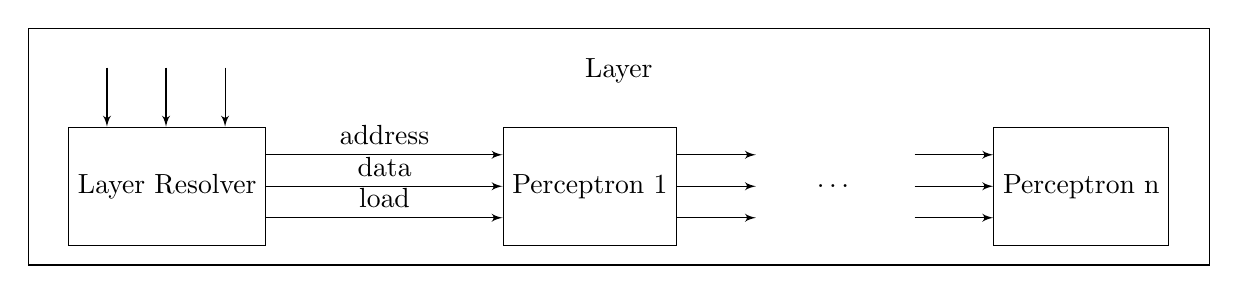
\begin{tikzpicture} [>=latex', node distance = 2cm]
            % Set primary nodes
            \tikzset{
                entity/.style={
                        rectangle,
                        draw
                    }
            }
            \tikzset{
                layerNode/.style={
                        draw,
                        rectangle,
                        minimum height=3cm,
                        minimum width=15cm,
                        text depth = 2cm
                    }
            }
            \tikzset{
                layerResolverNode/.style={
                        draw,
                        rectangle,
                        minimum height=1.5cm,
                        minimum width=2.5cm,
                    }
            }
            \tikzset{
                perceptronNode/.style={
                        draw,
                        rectangle,
                        minimum height=1.5cm,
                        minimum width=2cm,
                    }
            }
            % Configure arrows
            \tikzstyle{arrow} = [thick, ->, >=stealth]
            % Placing nodes
            \node[layerNode](layer){Layer};
            \node[layerResolverNode, right = 0cm of layer, xshift = -14.5cm, yshift = -0.5cm](layerResolver){Layer Resolver};
            \node[perceptronNode, right = 3cm of layerResolver](perceptron1){Perceptron 1};
            \node[perceptronNode, right = 1cm of perceptron1, draw=none](perceptron2){\dots};
            \node[perceptronNode, right = 1cm of perceptron2](perceptron3){Perceptron n};
            % Draw arrows
            \draw[->](layer.north) ++(-6.5,-0.5) -- ++(0,-0.75);
            \draw[->](layer.north) ++(-5.75,-0.5) -- ++(0,-0.75);
            \draw[->](layer.north) ++(-5,-0.5) -- ++(0,-0.75);
            \draw[->](layerResolver.east) ++(0,0.4) -- ++(3,0) node[midway,sloped,yshift=0.25cm]{address};
            \draw[->](layerResolver.east) ++(0,0) -- ++(3,0) node[midway,sloped,yshift=0.25cm]{data};
            \draw[->](layerResolver.east) ++(0,-0.4) -- ++(3,0) node[midway,sloped,yshift=0.25cm]{load};
            \draw[->](perceptron1.east) ++(0,0.4) -- ([yshift=0.4cm]perceptron2.west);
            \draw[->](perceptron1.east) -- (perceptron2.west);
            \draw[->](perceptron1.east) ++(0,-0.4) -- ([yshift=-0.4cm]perceptron2.west);
            \draw[->](perceptron2.east) ++(0,0.4) -- ([yshift=0.4cm]perceptron3.west);
            \draw[->](perceptron2.east) -- (perceptron3.west);
            \draw[->](perceptron2.east) ++(0,-0.4) -- ([yshift=-0.4cm]perceptron3.west);
        \end{tikzpicture}
        \caption{Layer Level Hardware Model}
        \label{fig:layerHardwareModel}
    \end{center}
\end{figure}
\FloatBarrier
In abbildung \ref{fig:layerHardwareModel} ist einer der 16 Layer grafisch dargestellt.
Zu sehen ist, dass die Leitungen: "address", "data" und "load" jedes Perceptron miteinander
verbindet und somit eine vollständige Adressierung und Datenbeaufschlagung garantiert wird.
\pagebreak
\section{Modul-Implementierung}
Im folgenden wird die Implemetierung der einzelnen Module basierend auf der 
Hardware-übersicht beschrieben.
\subsection{Top Level Resolver}
Der "Top Level Resolver" realisiert eine Aufteilung und Skalierung der Signale von dem 
Eingang des Systems zu den Modulen "Storage" und "Layer Resolver". Konkret bedeutet
das, dass wenn über die Signalleitung "mode" eine logische '1' anliegt die einzelnen 
schichten und somit die Perzeptronen adressiet werden. Liegt jedoch eine logische '0'
an dem Eingang des "Top Level Resolver" an, so wird der Speicher, welcher die späteren
Funktions-Werte des Systems enthält, adressiert.
\begin{figure}[htb!]
    \begin{center}
      \includegraphics[width=13.25cm]{ModuleDescription/top_level_resolver.png}
    \end{center}
    \caption{Modulbeschreibung "Top Level Resolver"} \label{fig:top_level_resolver}
  \end{figure}
\FloatBarrier
In Abbildung \ref{fig:top_level_resolver} ist die Modulbeschreibung dargestellt.
Daraus ist ersichtlich, dass die Datenleitung, welche an die einzelnen "Layer Resolver"-Module
geleitet wird in eine 4Bit-Datenleitung gekürzt wird. Des weiteren wird die Adressleitung
für das "Storage"-Modul in eine 10Bit-Datenleitung gekürzt. Daraus ergibt sich die Möglichkeit
1280 verschiedene 4Bit-Datenregister für die Perzeptron-Schichten und 1024 verschiedene
16Bit-Register für die Funktionseingabe in der erstem Perceptron-Schicht zu realisieren.
\begin{figure}[htbp]
\begin{lstlisting}[style=VHDL,numbers=left,stepnumber=1,basicstyle=\footnotesize]
behaviour : process (reset, mode, address_in, data_in, load_in) is
  begin
    if reset = '1' then
      ----------------------------------------------
      -- Reset all Outputs and internal Variables --
      ----------------------------------------------
      address_out_layer   <= (others => '0');
      data_out_layer      <= (others => '0');
      load_out_layer      <= '0';
      address_out_storage <= (others => '0');
      data_out_storage    <= (others => '0');
      load_out_storage    <= '0';
    elsif reset = '0' then
      ------------------
      -- Layer Branch --
      ------------------
      if mode = '0' then
        address_out_layer <= address_in;
        data_out_layer    <= data_in(3 downto 0); -- least significant bits
        load_out_layer    <= load_in;
        ---------------------------
        -- All others to default --
        ---------------------------
        address_out_storage <= (others => '0');
        data_out_storage    <= (others => '0');
        load_out_storage    <= '0';
        --------------------
        -- Storage Branch --
        --------------------
      elsif mode = '1' then
        address_out_storage <= address_in(9 downto 0); -- least significant bits
        data_out_storage    <= data_in;
        load_out_storage    <= load_in;
        ---------------------------
        -- All others to default --
        ---------------------------
        address_out_layer <= (others => '0');
        data_out_layer    <= (others => '0');
        load_out_layer    <= '0';
      end if;
    end if;
  end process;
\end{lstlisting}
\caption{Programmcode zu "Top Level Resolver"} \label{code:top_level_resolver}
\end{figure}
\FloatBarrier
In dem Programmcode aus \ref{code:top_level_resolver} ist ersichtlich, dass es sich lediglich
um rein kombinatorische Logik handelt, welche keinen externen Takt benötigt. Es handelt 
sich bei dem gezeigten Code lediglich um den "Process", die "Entity" und "Architecture"
sind in der Modulbeschreibung \ref{fig:top_level_resolver} ersichtlich.
\pagebreak
\subsection{Storage}
Das Modul "Storage" ist für die Speicherung der Eingangs-Funktionswerte zuständig, um das 
Modell des Multilayer-Perzeptrons mit Daten zu versorgen und Optimierungen auf bestimmte 
Funktionen vor zu nehmen.
\begin{figure}[htb!]
    \begin{center}
      \includegraphics[width=13.25cm]{ModuleDescription/storage.png}
    \end{center}
    \caption{Modulbeschreibung "Layer Resolver"} \label{fig:storage}
  \end{figure}
\FloatBarrier
\pagebreak
In der Modulbeschreibung aus Abbildung \ref{fig:storage} ist ersichtlich, dass der 
Speicher eine Adressweite von 10Bit besitzt und 16Bit Werte speichern kann. Des weiteren 
wird aus dem Code in Abbildung \ref{code:storage} ersichtlich, dass bei anlegen eines Taktsignals  "clk" 
die gespeicherten Werte iterativ am Ausgang \linebreak "layer\_output" ausgegeben werden. Der 
"layer\_output" stellt  die Verbindung zwischen dem Speichermodul und der ersten 
Perzeptron-Schicht dar.
\begin{figure}[htbp]
\begin{lstlisting}[style=VHDL,numbers=left,stepnumber=1,basicstyle=\footnotesize]
    behaviour : process (load_in_storage, clk, reset)
    variable count : integer range 0 to 1023;
  begin
    --------------------
    -- reset handling --
    --------------------
    if (reset = '1') then
      -- Reset the 16Bit values of the whole 10Bit long array.
      for i in 0 to 1023 loop
        stored_value(i) <= (others => '0');
        count := 0;
      end loop;
    end if;
    --------------------
    -- input handling --
    --------------------
    if (load_in_storage = '1') then
      -- If the load is triggered, safe the value at the address.
      stored_value(to_integer(unsigned(address_in_storage))) <= data_in_storage;
    end if;
    ---------------------
    -- output handling --
    ---------------------
    if (clk = '1') then
      layer_output <= stored_value(count);
      count := count + 1;
      if (count = 1023) then
        count := 0;
      end if;
    end if;
  end process;
\end{lstlisting}
\caption{Programmcode zu "Storage"} \label{code:storage}
\end{figure}
\pagebreak
\subsection{Layer Resolver}
Der "Layer Resolver" übernimmt die Rolle des Bindegliedes zwischen dem "Top Level Resolver"
und den einzelnen Schichten mit Perzeptronen.
\begin{figure}[htb!]
    \begin{center}
      \includegraphics[width=13.25cm]{ModuleDescription/layer_resolver.png}
    \end{center}
    \caption{Modulbeschreibung "Layer Resolver"} \label{fig:layer_resolver}
  \end{figure}
\FloatBarrier
In der Modulbeschreibung aus Abbildung \ref{fig:layer_resolver} ist ersichtlich, dass der 
"Layer Resolver" bei seiner Instanziierung einen Parameter übergeben bekommt, welcher angibt 
in welcher Schicht sich der "Layer Resolver" befindet. Dies ist nötig, um die Adressen richtig 
an die Perzeptronen in jeder einzelnen Schicht weiter zu leiten. Die 11Bit Eingangs-Adresse 
wird durch den "Layer Resover" in eine 7Bit Ausgangs-Adresse gewandelt.
\begin{figure}[htbp]
\begin{lstlisting}[style=VHDL,numbers=left,stepnumber=1,basicstyle=\footnotesize]
behaviour : process (address_in, reset, load_in, data_in) is
variable perceptron_address : integer range 0 to 15;
  begin
    if reset = '1' then
      address_out <= (others => '0');
      data_out    <= (others => '0');
      load_out    <= '0';
    else
      --------------------------
      -- detect valid address --
      --------------------------
      if (load_in = '1') then
        -- address = xxxx xxxx xxx 
        -- (layer, perceptron in layer, value)
        if (shift_right((unsigned(address_in) and "11110000000"), 7) = layer_count) then
          ------------------------------
          -- forward address and data --
          ------------------------------
          address_out <= address_in(6 downto 0);
          data_out    <= data_in;
          load_out    <= load_in;
        else
          -----------------------------------
          -- reset address and data output --
          -----------------------------------
          address_out <= (others => '0');
          data_out    <= (others => '0');
          load_out    <= '0';
        end if;
      end if;
    end if;
  end process;
\end{lstlisting}
\caption{Programmcode zu "Layer Resolver"} \label{code:layer_resolver}
\end{figure}
\FloatBarrier
Es handelt sich weider um einen rein kombinatorischen Prozess ohne Taktabhandlung.
\subsection{Perzeptron}
Das Perzeptron selbst besteht aus einer binären Eingabesteuerung anstelle von 
Gleitkommaberechnungen. Das bedeutet, dass die Verbindung von einem Perzeptron-Ausgang zu 
einem anderen Perzeptron-Eingang nur aktiv oder nicht aktiv sein kann.
Darüber hinaus ist der zweite Parameter innerhalb des Perzeptrons die Aktivierungsfunktion,
welche im Grunde die Summation über die "high"-Eingangs-signale darstellt.
Wenn die Summe größer ist als ein gegebener Wert wird der Ausgang des Perzeptrons auf 
"high" gesetzt. In dem Programmcode aus Abbildung \ref{code:perceptron} ist ersichtlich, 
dass die Adressierung des 16Bit-Vektors für die Gewichtung der Eingänge (aktiv oder nicht 
aktiv) auf insgesamt vier 4Bit-Vektoren aufgeteilt wird, welche von dem Perzeptron 
schließlich zu einem 16Bit-Vektor zusammengefasst werden. Die Adresierung des 
"activation\_value", welcher eine Aussage darüber trifft, ab wie vielen logischen "high"-
Werten der Ausgang eine "1" annimt wird auf die selbe Weise adressiert. Über die 
"data"-Verbindung wird schließlich den adressierten Speichern ein Wert zugewiesen.
Zusammenfasend ist zu sagen, dass die letzten 3-Bit in der Adresse immer die Adressierung 
der spezifischen Aktivierungs- und Sensitivitäts-funktionen darstellt.
\begin{figure}[htb!]
    \begin{center}
      \includegraphics[width=13.25cm]{ModuleDescription/perceptron.png}
    \end{center}
    \caption{Modulbeschreibung "Perzeptron"} \label{fig:perceptron}
  \end{figure}
\FloatBarrier
\begin{figure}[htbp]
\begin{lstlisting}[style=VHDL,numbers=left,stepnumber=1,style=myCustomMatlabStyle,basicstyle=\footnotesize]
behaviour : process (load, reset, dentrid_port, address, data) is
    variable count     : unsigned(3 downto 0)           := (others => '0');
    variable old_value : std_logic_vector (15 downto 0) := (others => '0');
  begin
    --------------------
    -- reset handling --
    --------------------
    if (reset = '1') then
      axon_port         <= '0';
      activation_value  <= (others => '1');
      sensitivity_value <= (others => '0');
      sens_1            <= (others => '0');
      sens_2            <= (others => '0');
      sens_3            <= (others => '0');
      sens_4            <= (others => '0');
      count     := (others         => '0');
      old_value := (others         => '0');
    else
      ----------------------------
      -- value storage handling --
      ----------------------------
      if load = '1' then
        -- check if the current perceptron is meant (first 4 Bit)
        if (shift_right((unsigned(address) and "1111000"), 3) = perceptron_id) then
          -- check the parameters (last 3 Bit)
          if ((unsigned(address) and "0000111") = 0) then
            activation_value <= unsigned(data);
          end if;
          if ((unsigned(address) and "0000111") = 1) then
            sens_1 <= unsigned(data);
          end if;
          if ((unsigned(address) and "0000111") = 2) then
            sens_2 <= unsigned(data);
          end if;
          if ((unsigned(address) and "0000111") = 3) then
            sens_3 <= unsigned(data);
          end if;
          if ((unsigned(address) and "0000111") = 4) then
            sens_4 <= unsigned(data);
          end if;
        end if;
        sensitivity_value <= sens_4 & sens_3 & sens_2 & sens_1;
      end if;
      ---------------------
      -- output handling --
      ---------------------
      if dentrid_port /= old_value then
        -- count over all Bits and proceed sensitivity and and output activation
        count := "0000";
        for i in 0 to 15 loop
          if ((dentrid_port(i) = '1') and (sensitivity_value(i) = '1')) then
            count := count + 1;
          end if;
        end loop; -- counter
        old_value := dentrid_port;
        -- update axon
        if (count >= activation_value) then
          axon_port <= '1';
        else
          axon_port <= '0';
        end if;
      end if;
    end if;
  end process;
\end{lstlisting}
\caption{Programmcode zum "Perzeptron"} \label{code:perceptron}
\end{figure}
\section{Gesamt-Implementierung}\label{sec:implementation}
Im folgenden wird die Gesamtimplementierung basierend auf der Hardwareübersicht erläutert
dabei wird lediglich auf die Instanziierung der Module eingegangen.
\begin{figure}[htb!]
    \begin{center}
      \includegraphics[width=13.25cm]{ModuleDescription/top_level_entity.png}
    \end{center}
    \caption{Modulbeschreibung "Top Level Entity"} \label{fig:top_level_entity}
  \end{figure}
\FloatBarrier
In der Abbildung \ref{fig:top_level_entity} ist die Beschreibung der oberen Instanz
des Systems beschrieben. Diese generiert alle weiteren Module und stellt deren Verbindung 
untereinander dar. Wie diese Verbindung realisiert ist wird im folgenden erläutert.
\pagebreak
\begin{figure}[htbp]
\begin{lstlisting}[style=VHDL,numbers=left,stepnumber=1,style=myCustomMatlabStyle,basicstyle=\footnotesize]
----------------------
-- Internal Signals --
----------------------
-- connection top level resolver to layer
signal address_int_layer : std_logic_vector(10 downto 0) := (others => '0'); 
signal data_int_layer    : std_logic_vector(3 downto 0)  := (others => '0');
signal load_int_layer    : std_logic                     := '0';
-- connection top level resolver to storage
signal address_int_storage : std_logic_vector(9 downto 0)  := (others => '0');
signal data_int_storage    : std_logic_vector(15 downto 0) := (others => '0');
signal load_int_storage    : std_logic                     := '0';
-- connect storage to first layer
signal storage_to_first_layer : std_logic_vector(15 downto 0) := (others => '0');
-- layer connection arrays
-- axon ports to next layer
type arr_16_times_16 is array (0 to 14) of std_logic_vector(15 downto 0);
signal layer_axon_arr : arr_16_times_16;
-- address from layer resolver to layer
type arr_16_times_7 is array (0 to 15) of std_logic_vector(6 downto 0);
signal address_layer_arr : arr_16_times_7;
-- data from layer resolver to layer
type arr_16_times_4 is array (0 to 15) of std_logic_vector(3 downto 0);
signal data_layer_arr : arr_16_times_4;
-- load from layer resolver to layer
signal load_layer : std_logic_vector (15 downto 0);
\end{lstlisting}
\caption{Programmcode der internen Signale} \label{code:internal_signals}
\end{figure}
\begin{figure}[htb!]
    \begin{center}
      \includegraphics[width=13.25cm]{ModuleDescription/internal_signals1.png}
    \end{center}
    \caption{Beschreibung der internen Signale der "Top Level Entity"} \label{fig:internal_signals1}
  \end{figure}
\FloatBarrier
\begin{figure}[htb!]
    \begin{center}
      \includegraphics[width=13.25cm]{ModuleDescription/internal_signals2.png}
    \end{center}
    \caption{Fortführung der Beschreibung der internen Signale der "Top Level Entity"} \label{fig:internal_signals2}
  \end{figure}
\FloatBarrier
In Abbildung \ref{fig:internal_signals1} und \ref{fig:internal_signals2} sind die
internen Signale, welche zur Verbindung der Module nötig sind beschrieben.
Alle internen Signale wurden kompatibel zu den Schnittstellen angelegt.
Die jeweilige Verbindung einer Perzeptron-Schicht mit der nächsten im Bezug auf 
die Daten- und Adressleitung wird jeweils durch ein 2-dimensionales "Array" aus 
16Bit Vektoren realisiert.
\pagebreak
\subsection{Instanziierung Der layer}
Im folgenden wird lediglich auf die Instanziierung der Layer eingegeangen. 
Die Instanziierung der restlichen Module funktioniert ähnlich dem der einzelnen Layer.
\begin{figure}[htbp]
\begin{lstlisting}[style=VHDL,numbers=left,stepnumber=1,style=myCustomMatlabStyle,basicstyle=\footnotesize]
-- instances of layer resolver
layer_resolvers : for i in 0 to 15 generate -- generate 16 layer resolvers
  layer_resolvers_inst : layer_resolver
  generic map(
    layer_count => i
  )
  port map(
    reset       => reset,
    address_in  => address_int_layer, -- tlr to resolvers
    data_in     => data_int_layer, -- ""
    load_in     => load_int_layer, -- ""
    address_out => address_layer_arr(i), -- layer resolver to perceptron array
    data_out    => data_layer_arr(i), -- ""
    load_out    => load_layer(i)
  );
end generate;
-- two dimensional layer array of perceptrons 14 x 16 (layer x perceptron)
layer_arr_2D : for i in 1 to 14 generate -- layer
  layer_arr_1D : for j in 0 to 15 generate -- perceptron in layer
    perceptron_arr_inst : perceptron
    generic map(
      perceptron_id => j
    )
    port map(
      reset        => reset,
      dentrid_port => layer_axon_arr(i - 1), -- prev layer to current layer
      axon_port    => layer_axon_arr(i)(j), -- current to next layer
      address      => address_layer_arr(i), -- layer resolver to perceptron array
      data         => data_layer_arr(i), -- ""
      load         => load_layer(i) -- ""
    );
  end generate;
end generate;
\end{lstlisting}
\caption{Programmcode der internen Signale} \label{code:generate_layers}
\end{figure}
\FloatBarrier
In der Abbildung \ref{code:generate_layers} ist zu sehen, dass insgesamt 16 
"layer\_resolver" und 13 Schichten mit Perzeptronen instanziiert werden. In jeder 
Perzeptron-Schicht befinden sich wiederum jeweils 16 Perzeptronen. Wie bereits in 
Abschnitt \ref{sec:implementation} erwähnt, werden die erzeugten Pereptronen
bei der Instanziierung mit den internen Signalen verbunden.
\pagebreak
\section{Validierung}
Die Validierung der einzelnen Module, der Integration verschiedener Module und der
des gesamten Systems wird mit Hilfe der Simulation auf Regeister-Transfer-Ebene 
in "Modelsim" realisiert. Alle Tests können durch hinzufügen der benötigten Module 
und das Ausführen der Modelsim-Skripte mit der Endung .do ausgeführt werden.
Die erwähnten Skripte befinden sich im Ordner "SimulationConf".
\subsection{Modultest}
Im Folgenden werden die Modultests zu allen Modulen erläutert.
\subsubsection{Top Level Resolver}
Der "Top Level Resolver" wird mit besonderem Augenmerk auf seine Reaktion auf die
verschiedenen Modi untersucht. Er dient als Stellglied für die Weiterleitung und
Anpassung der Länge der Signale. Um die Funktion dahingehend zu überprüfen wurde 
folgender Ablauf innerhalb einer Testbench realisiert:
\begin{figure}[htbp]
\begin{lstlisting}[style=VHDL,numbers=left,stepnumber=1,style=myCustomMatlabStyle,basicstyle=\footnotesize]
beh_process : process
  begin
    reset      <= '1';
    mode       <= '0';
    address_in <= "00000000000";
    data_in    <= "0000000000000000";
    load_in    <= '0';
    wait for 2 * clk_period;
    reset <= '0';
    --------------------------
    mode       <= '0';
    load_in    <= '1';
    address_in <= "00101001001";
    data_in    <= "0000000000001101";
    wait for 2 * clk_period;
    ----------------------------
    -- addressing the storage --
    ----------------------------
    mode       <= '1';
    load_in    <= '1';
    address_in <= "01101100000";
    data_in    <= "0000000000000011";
    wait for 2 * clk_period;
    report "Simulation Stop";
    stop;
  end process;
\end{lstlisting}
\caption{Programmcode der "Top Level Resolver" Testbench} \label{code:tlr_testbench}
\end{figure}
\begin{figure}[htb!]
    \begin{center}
      \includegraphics[width=15cm]{SimulationPictures/top_level_resolver_sim.png}
    \end{center}
    \caption{Simulationsergebnis "Top Level Resolver"} \label{fig:tlr_sim}
  \end{figure}
\FloatBarrier
In dem Simulationsergebnis in Abbildung \ref{fig:tlr_sim} ist zu sehen, dass der 
"Top Level Resolver" das erwartete Verhalten erfüllt und die Signale je nach gewähltem 
"mode" weiter leitet. Des weiteren ist auch die Funktionalität der Bearbeitung der 
Signale im Bezug auf deren Länge erfüllt.
\pagebreak
\subsubsection{Storage}
Das Modul "Storage" wird auf seine Funktionalität im Bezug auf die Speicherung und Wiedergabe
von 16Bit-Zahlen geprüft. Dafür werden in einer Testumgebung Zahlen erzeugt, in den Speicher 
geschrieben und danach wieder iterativ ausgegeben.
\begin{figure}[htbp]
\begin{lstlisting}[style=VHDL,numbers=left,stepnumber=1,style=myCustomMatlabStyle,basicstyle=\footnotesize]
check_beh : process
begin
  -----------------
  -- first reset --
  -----------------
  reset              <= '1';
  clk                <= '0';
  load_in_storage    <= '0';
  address_in_storage <= std_logic_vector(to_unsigned(0, address_in_storage'length));
  data_in_storage    <= std_logic_vector(to_unsigned(0, data_in_storage'length));
  wait for clk_period;
  reset <= '0';
  --------------------------
  -- set the input values --
  --------------------------
  address_in_storage <= std_logic_vector(to_unsigned(0, address_in_storage'length));
  data_in_storage    <= std_logic_vector(to_unsigned(244, data_in_storage'length));
  wait for clk_period;
  load_in_storage <= '1';
  wait for clk_period;
  load_in_storage    <= '0';
  address_in_storage <= std_logic_vector(to_unsigned(1, address_in_storage'length));
  data_in_storage    <= std_logic_vector(to_unsigned(12, data_in_storage'length));
  wait for clk_period;
  load_in_storage <= '1';
  wait for clk_period;
  load_in_storage    <= '0';
  address_in_storage <= std_logic_vector(to_unsigned(2, address_in_storage'length));
  data_in_storage    <= std_logic_vector(to_unsigned(899, data_in_storage'length));
  wait for clk_period;
  load_in_storage <= '1';
  wait for clk_period;
  load_in_storage <= '0';
  ---------------------------
  -- get the output values --
  ---------------------------
  clk <= '1';
  wait for clk_period;
  clk <= '0';
  wait for clk_period;
  clk <= '1';
  wait for clk_period;
  clk <= '0';
  wait for clk_period;
  clk <= '1';
  wait for clk_period;
  clk <= '0';
  wait for clk_period;
  report "Simulation Stop";
  stop;
end process;
\end{lstlisting}
\caption{Programmcode der "Storage" Testbench} \label{code:storage_testbench}
\end{figure}
\pagebreak
\begin{figure}[htb!]
    \begin{center}
      \includegraphics[width=15cm]{SimulationPictures/storage_sim.png}
    \end{center}
    \caption{Simulationsergebnis "Storage"} \label{fig:storage_sim}
  \end{figure}
\FloatBarrier
\begin{figure}[htb!]
    \begin{center}
      \includegraphics[width=15cm]{SimulationPictures/storage_memory_sim.png}
    \end{center}
    \caption{Speicherwerte "Storage"} \label{fig:storage_memory_sim}
  \end{figure}
\FloatBarrier
In dem Simulationsergebnis aus Abbildung \ref{fig:storage_sim} ist zu sehen, dass die 
Funktionswerte korrekt am Ausgang nach dem Speichern ausgegeben werden. Außerdem wird 
der Speicher nach dem Zurücksetzen korrekt mit "0" gefüllt und die Werte ein weiteres
mal durch das Prüfen mit der Funktion "Memory Data" in "Modelsim", wie in Abbildung
\ref{fig:storage_memory_sim} zu sehen, geprüft.
\pagebreak
\subsubsection{Layer Resolver}
Der "Layer Resolver" hat die Funktion, die eingehenden Adress- und Datensignale auf die 
einzelnen Perzeptronen in der jeweiligen Schicht zu verteilen. Dies geschieht, wenn 
die richtige Adresse der jeweiligen Schicht codiert ist. In der folgenden Testbench
in Abbildung \ref{code:layer_resolver_testbench} wird dieses Verhalten geprüft.
\begin{figure}[htbp]
\begin{lstlisting}[style=VHDL,numbers=left,stepnumber=1,style=myCustomMatlabStyle,basicstyle=\footnotesize]
check_beh : process
  begin
    ---------------------------
    -- assign default values --
    ---------------------------
    address_in <= (others => '0');
    data_in    <= (others => '0');
    load_in    <= '0';
    -------------------
    -- trigger reset --
    -------------------
    reset <= '1';
    wait for 1.5 * clk_period;
    reset <= '0';
    -----------------------
    -- set first address --
    -----------------------
    -- adress format: xxxx xxxx xxx (layer, perceptron, value)
    load_in    <= '1';
    address_in <= "00000011010"; -- (0, 3, 2)
    data_in    <= std_logic_vector(to_unsigned(4, data_in'length));
    wait for clk_period;
    ------------------------
    -- set second address --
    ------------------------
    load_in    <= '1';
    address_in <= "00010011010"; -- (1, 3, 2)
    data_in    <= std_logic_vector(to_unsigned(5, data_in'length));
    wait for clk_period;
    -----------------------------------
    -- check the reset functionality --
    -----------------------------------
    reset <= '1';
    wait for 2 * clk_period;
    reset <= '0';
    stop;
  end process;
\end{lstlisting}
\caption{Programmcode der "Layer Resolver" Testbench} \label{code:layer_resolver_testbench}
\end{figure}
\begin{figure}[htb!]
    \begin{center}
      \includegraphics[width=15cm]{SimulationPictures/layer_resolver_sim.png}
    \end{center}
    \caption{Simulationsergebnis "Layer Resolver"} \label{fig:layer_resolver_sim}
  \end{figure}
\FloatBarrier
In dem Simulationsergebnis aus Abbildung \ref{fig:layer_resolver_sim} ist zu erkennen, dass
die Daten- und Adressignale lediglich dann weiter geleitet und im Fall der Adressleitung
gekürzt wird, sofern die richtige Schicht, in dem Fall die Schicht 1 adressiert wurde.
\pagebreak
\subsubsection{Perzeptron}
Das Modul "Perzeptron" realisiert die eigentliche Funktion des am Ende in der "Top Level 
Entity" gebildeten Netzes dieser. Die Testbench in Abbildung \ref{code:perceptron_testbench_1}
und \ref{code:perceptron_testbench_2} prüft, ob die Werte für die Eingangs-sensitivität
und den Schwellwert der Aktivierung gespeichert werden und schließlich auf Eingaben
basier-end auf den zuvor eingestellten Werten entsprechend reagiert wird.
\begin{figure}[htbp]
    \begin{lstlisting}[style=VHDL,numbers=left,stepnumber=1,style=myCustomMatlabStyle,basicstyle=\footnotesize]
check_beh : process
  begin
    --------------------
    -- default values --
    --------------------
    reset        <= '0';
    dentrid_port <= (others => '0');
    address      <= (others => '0');
    data         <= (others => '0');
    load         <= '0';
    wait for clk_period;
    reset <= '1';
    wait for clk_period;
    reset <= '0';
    wait for clk_period;
    --------------------------
    -- set activation value --
    --------------------------
    address <= "0000000";
    wait for clk_period;
    data <= "1111";
    wait for clk_period;
    load <= '1';
    wait for clk_period;
    load <= '0';
    wait for clk_period;
    -----------------------------
    -- set a sensitivity value --
    -----------------------------
    -- sens_1
    address <= "0000001";
    wait for clk_period;
    data <= "1111";
    wait for clk_period;
    load <= '1';
    wait for clk_period;
    load <= '0';
    wait for clk_period;
    -- sens_2
    address <= "0000010";
    wait for clk_period;
    data <= "1111";
    wait for clk_period;
    load <= '1';
    wait for clk_period;
    load <= '0';
    wait for clk_period;
\end{lstlisting}
\caption{Programmcode der "Perzeptron" Testbench} \label{code:perceptron_testbench_1}
\end{figure}
\FloatBarrier
\begin{figure}[htbp]
    \begin{lstlisting}[style=VHDL,numbers=left,stepnumber=1,style=myCustomMatlabStyle,basicstyle=\footnotesize]
    -- sens_3
    address <= "0000011";
    wait for clk_period;
    data <= "1111";
    wait for clk_period;
    load <= '1';
    wait for clk_period;
    load <= '0';
    wait for clk_period;
    -- sens_4
    address <= "0000100";
    wait for clk_period;
    data <= "1111";
    wait for clk_period;
    load <= '1';
    wait for clk_period;
    load <= '0';
    wait for clk_period;
    -- final load to set the sens value
    load <= '1';
    wait for clk_period;
    load <= '0';
    wait for clk_period;
    ------------------------------------------------------
    -- check the programmed values and output behaviour --
    ------------------------------------------------------
    dentrid_port <= "1111111111111111";
    wait for 2 * clk_period;
    dentrid_port <= "1111111111111110";
    wait for 2 * clk_period;
    dentrid_port <= "1111111111111111";
    wait for 2 * clk_period;
    report "Simulation Stop";
    stop;
  end process;  
\end{lstlisting}
\caption{Fortsetzung des Programmcode der "Perzeptron" Testbench} \label{code:perceptron_testbench_2}
\end{figure}
\FloatBarrier
\begin{figure}[htb!]
    \begin{center}
      \includegraphics[width=15cm]{SimulationPictures/perceptron_sim.png}
    \end{center}
    \caption{Simulationsergebnis "Perceptron"} \label{fig:perceptron_sim}
  \end{figure}
\FloatBarrier
In dem Simulationsergebnis in Abbildung \ref{fig:perceptron_sim} ist zu sehen, dass die
extern angelegten Signale intern gespeichert und ausgewertet werden. Auswerten meint
hierbei das Zusammenfügen der 4Bit-Datenleitung zu einem 16Bit-Eingangsvektor, welcher
die Sensitivität der Eingangssignale des Perzeptron festlegt. Des weiteren ist ersichtlich,
dass bei Anlegen eines der Sensitivität ("sensitivity\_value") und dem Aktivierungswert
("activation\_value") entsprechenden Eingangssignals der Ausgang eine logische "1"
ausgibt.
\pagebreak
\subsection{Integrationstest}
Bei dem Integrationstest wird geprüft, ob einzelne Module seitens der Schnittstelle 
zusammen spielen und die erwartete Funktion erfüllen.
\subsubsection{Top Level Resover und Storage}
Als Integrationstest wurde der "Top Level Resolver" und das Modul "Storage" zusammen 
geschaltet und auf korrekte Funktion überprüft. Dafür wurden wie in Abbildung 
\ref{code:tlr_storage_testbench1} zu sehen zufällige Werte für den Eingang verwendet.
\begin{figure}[htbp]
\begin{lstlisting}[style=VHDL,numbers=left,stepnumber=1,style=myCustomMatlabStyle,basicstyle=\footnotesize]
beh_process : process is
    -- randome number variable
    variable seed1, seed2 : integer := 999;
    -- randome vector number generator
    impure function rand_slv(len : integer) return std_logic_vector is
      variable r                   : real;
      variable slv                 : std_logic_vector(len - 1 downto 0);
    begin
      for i in slv'range loop
        uniform(seed1, seed2, r);
        if r > 0.5 then
          slv(i) := '1';
        else
          slv(i) := '0';
        end if;
      end loop;
      return slv;
    end function;
    ----------------------------
    -- actual behaviour check --
    ----------------------------
  begin
    -- reset everything and set standard values
    wait for clk_period;
    clk     <= '0';
    reset   <= '1';
    mode    <= '1'; -- '1' for storage addressing
    address <= (others => '0');
    data    <= (others => '0');
    load    <= '0';
    wait for clk_period;
    -- load some data in the storage
    reset <= '0';
    for i in 0 to 1023 loop
      -- addressing every place in the storage
      address <= std_logic_vector(to_unsigned(i, address'length));
      data    <= rand_slv(16); -- write some randome data in the storage
      wait for clk_period;
      load <= '1';
      wait for clk_period;
      load <= '0';
    end loop;
\end{lstlisting}
\caption{Programmcode der "Top Lavel Resolver" und "Storage" Testbench} \label{code:tlr_storage_testbench1}
\end{figure}
\begin{figure}[htbp]
\begin{lstlisting}[style=VHDL,numbers=left,stepnumber=1,style=myCustomMatlabStyle,basicstyle=\footnotesize]
  -- change to layer branch
  mode <= '0';
  wait for clk_period;
  for i in 0 to 1023 loop
    -- addressing every place in the storage
    address <= std_logic_vector(to_unsigned(i, address'length));
    data    <= rand_slv(16); -- write some randome data in the storage
    wait for clk_period;
    load <= '1';
    wait for clk_period;
    load <= '0';
  end loop;
  -- get the data back iteratively at the output port
  for i in 0 to 1023 loop
    wait for clk_period;
    clk <= '1';
    wait for clk_period;
    clk <= '0';
  end loop;
  stop;
end process;
\end{lstlisting}
\caption{Fortsetzung Programmcode der "Top Level Resolver" und "Storage" Testbench} \label{code:tlr_storage_testbench2}
\end{figure}
\FloatBarrier
\begin{figure}[htb!]
    \begin{center}
      \includegraphics[width=15cm]{SimulationPictures/tlr_storage_store_sim.png}
    \end{center}
    \caption{Simulationsergebnis weiterleitung Speicher "Top Lavel Resolver" und "Storage"} \label{fig:tlr_storage_sim1}
  \end{figure}
\FloatBarrier
In der Abbildung \ref{fig:tlr_storage_sim1} wurde im wesetlichen betrachtet, ob die 
Weiterleitung und Bearbeitung des eingehenden Signals auf das interne Signal-Routing
für den Speicher-Zweig seine Funktion erfüllt.
\begin{figure}[htb!]
    \begin{center}
      \includegraphics[width=15cm]{SimulationPictures/tlr_storage_layer_sim.png}
    \end{center}
    \caption{Simulationsergebnis weiterleitung Layer "Top Level Resolver" und "Storage"} \label{fig:tlr_storage_sim2}
  \end{figure}
\FloatBarrier
In der Abbildung \ref{fig:tlr_storage_sim2} wurde dies nun ebenfalls für den Layer-Zweig
betrachtet.
\begin{figure}[htb!]
    \begin{center}
      \includegraphics[width=15cm]{SimulationPictures/storage_memory_data_sim.png}
    \end{center}
    \caption{Speicherinhalt des "Storage" Moduls beim Integrationstes} \label{fig:storage_content}
  \end{figure}
\FloatBarrier
In der Abbildung \ref{fig:storage_content} ist der zufällige Speicherinhalt des "Storage"
Moduls abgebildet.
\pagebreak
\subsection{Systemtest}
In Abbildung \ref{code:top_level_entity_testbench1} ist der Programmcode zum testen der
"Top Level Entity" ersichtlich. Zunächst werden einige Zufallswerte in den Speicher
geschrieben, um im späteren Verlauf eine Stimulation des Multilayer-Perzeptrons 
zu realisieren. Danach wird mit den standard Aktivierungs- und Sensitivitätswerten
diese Stimulation einmal komplett über alle Funktionswerte iteriert. Darauffolgend
werden, wie in Abbildung \ref{code:top_level_entity_testbench1} zu sehen, nun zufällige 
Werte für die Aktivierungs- und Sensitivitätswerte generiert, und adressiert. 
Schließlich werden die im Speicher abgelegten Werte wieder iteriert, um das jetzt sich 
ergebende Verhalten ebenfalls zu untersuchen.
\begin{figure}[htbp]
\begin{lstlisting}[style=VHDL,numbers=left,stepnumber=1,style=myCustomMatlabStyle,basicstyle=\footnotesize]
-- system integration test
  beh_process : process
    -- randome number variable
    variable seed1, seed2 : integer := 999;
    -- randome vector number generator
    impure function rand_slv(len : integer) return std_logic_vector is
      variable r                   : real;
      variable slv                 : std_logic_vector(len - 1 downto 0);
    begin
      for i in slv'range loop
        uniform(seed1, seed2, r);
        if r > 0.5 then
          slv(i) := '1';
        else
          slv(i) := '0';
        end if;
      end loop;
      return slv;
    end function;
  begin
    --------------------------------
    -- Write Test Data to Storage --
    --------------------------------
    -- reset everything and set standard values
    wait for clk_period;
    clk     <= '0';
    reset   <= '1';
    mode    <= '1'; -- '1' for storage addressing
    address <= (others => '0');
    data    <= (others => '0');
    load    <= '0';
    wait for clk_period;
    -- load some data in the storage
    reset <= '0';
    for i in 0 to 1023 loop
      -- addressing every place in the storage
      address <= std_logic_vector(to_unsigned(i, address'length));
      data    <= rand_slv(16); -- write some randome data in the storage
      wait for clk_period;
      load <= '1';
      wait for clk_period;
      load <= '0';
    end loop;
    ------------------------------------------------
    -- Standard Activation and Sensitivity Values --
    ------------------------------------------------
    -- get the storage data back iteratively at the output port
    for i in 0 to 1023 loop
      wait for clk_period;
      clk <= '1';
      wait for clk_period;
      clk <= '0';
    end loop;
\end{lstlisting}
\caption{Programmcode der "Top Level Entity" Testbench} \label{code:top_level_entity_testbench1}
\end{figure}
\FloatBarrier
\begin{figure}[htbp]
\begin{lstlisting}[style=VHDL,numbers=left,stepnumber=1,style=myCustomMatlabStyle,basicstyle=\footnotesize]
    ----------------------------------------------------
    -- Non Standard Activation and Sensitivity Values --
    ----------------------------------------------------
    -- format is: xxxx xxxx xxx (layer, perceptron in layer, value)
    -- value => 0 = activation value, 1-4 = sens_1 to sens_4,
    -- ends up in 16Bit activation vector
    mode <= '0'; -- '0' for layer addressing
    for i in 0 to 2047 loop -- iterate over all perceptrons
      address <= std_logic_vector(to_unsigned(i, address'length));
      data    <= "0000000000001111" and rand_slv(16); -- set randome activation value
      wait for clk_period/2;
      load <= '1';
      wait for clk_period/2;
      load <= '0';
    end loop;
    -- get the storage data back iteratively at the output port
    for i in 0 to 1023 loop
      wait for clk_period;
      clk <= '1';
      wait for clk_period;
      clk <= '0';
    end loop;
    stop;
  end process;
\end{lstlisting}
\caption{Fortsetzung Programmcode der "Top Level Entity" Testbench} \label{code:top_level_entity_testbench2}
\end{figure}
\FloatBarrier
\begin{figure}[htb!]
    \begin{center}
      \includegraphics[width=15cm]{SimulationPictures/top_level_entyity_sens_sim.png}
    \end{center}
    \caption{Systemtest zum Speichern von Aktivierungs- und Sensitivitätswerten} \label{fig:system_params}
  \end{figure}
\FloatBarrier
In der Abbildung \ref{fig:system_params} ist unter dem "Divider" mit Namen: "Perceptron 
Signals" der Signalverlauf innerhalb der ersten Instanz des Perzeptron in dem ersten 
"Layer" zu sehen. Es ist ersichtlich, dass dieses Perzeptron die gegebenen Werte 
zur Sensitivität und Aktivierung übernimmt und in den internen Speicher ablegt.
\begin{figure}[htb!]
    \begin{center}
      \includegraphics[width=15cm]{SimulationPictures/top_level_entity_stimulus_sim.png}
    \end{center}
    \caption{Systemtest zur Reaktion auf Eingags-Stimuli} \label{fig:system_stimuli}
  \end{figure}
\FloatBarrier
In der Abbildung \ref{fig:system_stimuli} ist ersichtlich, dass das System auf ein
Stimuli am Eingang entsprechend reagiert und die Ausgänge des "Axon-Port" setzt.
Dies ist unter dem "Divider" mit dem Namen "Perceptron Layer" innerhalb des 
"layer\_axon\_arr" ersichtlich.
\pagebreak
\subsection{Timing-Analyse}
Das Skript für die Timing-Analyse befindet sich in dem Ordner quartus/simulation/modelsim
und trägt den Namen "perceptron\_on\_FPGA\_run\_msim\_gate\_vhdl.do". Leider ist mein Rechner 
nicht in der Lage dieses Skript in absehbarer Zeit zu simulieren, daher sei hier lediglich
der Verweis auf dieses angegeben.

\section{Zusammenfassung und Ausblick}
Zum Schluss sei erwähnt, dass das Multilayer-Perzeptron bis zum endgültigen Hardware-Test 
weitere Systemtest durchlaufen sollte, hinsichtlich der Korektheit von Eingaben und 
zu erwartenden Ausgaben. Darüber hinaus ist die Implementierung eines Optimierungs-
Algorithmus für das Anlernen des Systems notwendig. Des weiteren sei erwähnt, dass die 
Implementierung des Speichers überarbeitet werden sollte, da bei nicht einhalten von 
äußeren Timing- Vorgaben hier unerwartetes Verhalten auftreten kann. Ein Umschalten 
zwischen schreiben und lesen des Speichers ist an dieser Stelle sinnvoller, als das 
Abhandeln von zwei verschiedenen Takt-Leitungen für lesen und schreiben des Speichers.

\section{Eigenständigkeitserklärung}
Hiermit bestätige ich, dass ich die vorliegende Arbeit selbständig verfasst und keine 
anderen als die angegebenen Hilfsmittel benutzt habe. Die Stellen der Arbeit, die dem 
Wortlaut oder dem Sinn nach anderen Werken einschließlich Internetquellen entnommen sind, 
wurden unter Angabe der Quelle kenntlich gemacht.
\linebreak
\linebreak
\linebreak
\linebreak
Fabian Franz
\end{document}